%!TEX program = xelatex
\documentclass[dvipsnames, svgnames,a4paper,11pt]{article}
% ----------------------------------------------------
%   中山大学物理与天文学院本科实验报告模板
%   作者:Huanyu Shi,2019级
%   知乎:https://www.zhihu.com/people/za-ran-zhu-fu-liu-xing
%   Github:https://github.com/huanyushi/SYSU-SPA-Labreport-Template
%   Last update : 2023.4.10
% ----------------------------------------------------

% ----------------------------------------------------- 
%	加边框的命令
%	参考:https://tex.stackexchange.com/questions/531559/how-to-add-the-page-border-for-first-two-pages-in-latex
\usepackage{tikz}
\usetikzlibrary{calc}
\usepackage{eso-pic}
\AddToShipoutPictureBG{%
\begin{tikzpicture}[overlay,remember picture]
\draw[line width=0.6pt] % 边框粗细
    ($ (current page.north west) + (0.6cm,-0.6cm) $)
    rectangle
    ($ (current page.south east) + (-0.6cm,0.6cm) $); % 边框位置
\end{tikzpicture}}


\usepackage{xcolor}
\definecolor{c1}{HTML}{2752C9} % 目录颜色
\definecolor{c2}{RGB}{190,20,83} % 引用颜色

\usepackage{ctex}
\usepackage[top=28mm,bottom=28mm,left=15mm,right=15mm]{geometry}
\usepackage{hyperref} 
\hypersetup{
	colorlinks,
	linktoc = section, % 超链接位置,选项有section, page, all
	linkcolor = c1, % linkcolor 目录颜色
	citecolor = c1  % citecolor 引用颜色
}
\usepackage{amsmath,enumerate,multirow,float}
\usepackage{tabularx}
\usepackage{tabu}
\usepackage{subfig}
\usepackage{fancyhdr}
\usepackage{graphicx}
\usepackage{wrapfig}  
\usepackage{physics}
\usepackage{appendix}
\usepackage{amsfonts}

%
\usepackage{tcolorbox}
\tcbuselibrary{skins,breakable}
\newtcolorbox{tbox}[2][]{
    colframe=black!70!,
    breakable,
    enhanced,
	boxrule =0.5pt,
    title = {#2},
    fonttitle = \large\kaishu\bfseries,
	drop fuzzy shadow,
    #1
}
\newtcolorbox[auto counter,number within=section]{question}[1][]{
  top=2pt,bottom=2pt,arc=1mm,
  boxrule=0.5pt,
%   frame hidden,
  breakable,
  enhanced, %跨页后不会显示下边框
  coltitle=c1!80!gray,
  colframe=c1,
  colback=c1!3!white,
  drop fuzzy shadow,
  title={思考题~\thetcbcounter:\quad},
  fonttitle=\bfseries,
  attach title to upper,
  #1
}

% ---------------------------------------------------------------------
%	利用cleveref改变引用格式,\cref是引用命令
\usepackage{cleveref}
\crefformat{figure}{#2{\textcolor{c2}{图 #1}}#3} % 图片的引用格式
\crefformat{equation}{#2{(\textcolor{c2}{#1})}#3} % 公式的引用格式
\crefformat{table}{#2{\textcolor{c2}{表 #1}}#3} % 表格的引用格式


% ---------------------------------------------------------------------
%	页眉页脚设置
\fancypagestyle{plain}{\pagestyle{fancy}}
\pagestyle{fancy}
\lhead{\kaishu 中山大学物理与天文学院近代物理实验\uppercase\expandafter{\romannumeral1}} % 左边页眉,学院 + 课程
\rhead{\kaishu D8 \quad 氦氖激光综合实验} % 右边页眉,实验报告标题
\cfoot{\thepage} % 页脚,中间添加页码


% ---------------------------------------------------------------------
%	对目录、章节标题的设置
\renewcommand{\contentsname}{\centerline{\huge 目录}}
\usepackage{titlesec}
\usepackage{titletoc}
% \titleformat{章节}[形状]{格式}{标题序号}{序号与标题间距}{标题前命令}[标题后命令]
\titleformat{\section}{\centering\LARGE\songti}{}{1em}{}

% ---------------------------------------------------------------------
%   listing代码环境设置
\usepackage{listings}
\lstloadlanguages{python}
\lstdefinestyle{pythonstyle}{
backgroundcolor=\color{gray!5},
language=python,
frameround=tftt,
frame=shadowbox, 
keepspaces=true,
breaklines,
columns=spaceflexible,                   
basicstyle=\ttfamily\small, % 基本文本设置,字体为teletype,大小为scriptsize
keywordstyle=[1]\color{c1}\bfseries, 
keywordstyle=[2]\color{Red!70!black},   
stringstyle=\color{Purple},       
showstringspaces=false,
commentstyle=\ttfamily\scriptsize\color{green!40!black},%注释文本设置,字体为sf,大小为smaller
tabsize=2,
morekeywords={as},
morekeywords=[2]{np, plt, sp},
numbers=left, % 代码行数
numberstyle=\it\tiny\color{gray}, % 代码行数的数字字体设置
stepnumber=1,
rulesepcolor=\color{gray!30!white}
}




% ---------------------------------------------------------------------
%	其他设置
\def\degree{${}^{\circ}$} % 角度
\graphicspath{{./images/}} % 插入图片的相对路径
\allowdisplaybreaks[4]  %允许公式跨页 % 导入模板的相关设置
\usepackage{lipsum}
\usepackage{enumitem}
\usepackage{tabularray}  %绘制表格时可以更加方便添加框线
\setlist[enumerate]{label=\textup{(\arabic*)}}



%---------------------------------------------------------------------
%	正文
%---------------------------------------------------------------------

\begin{document}


\begin{table}
	\renewcommand\arraystretch{1.7}
	\begin{tabularx}{\textwidth}{
		|X|X|X|X
		|X|X|X|X|}
	\hline
	\multicolumn{2}{|c|}{预习报告}&\multicolumn{2}{|c|}{实验记录}&\multicolumn{2}{|c|}{分析讨论}&\multicolumn{2}{|c|}{总成绩}\\
	\hline
	\LARGE25 & & \LARGE30 & & \LARGE25 & & \LARGE80 & \\
	\hline
	\end{tabularx}
\end{table}


\begin{table}
	\renewcommand\arraystretch{1.7}
	\begin{tabularx}{\textwidth}{|X|X|X|X|}
	\hline
	专业:& 物理学 &年级:& 2022级\\
	\hline
	姓名:& 戴鹏辉  & 学号: & 2344016 \\
	\hline
	日期:& 2024/9/20 & 教师签名:& \\
	\hline
	\end{tabularx}
\end{table}

\begin{center}
	\LARGE D1 \quad 锁相放大器与弱信号测量
\end{center}

\textbf{【实验报告注意事项】}
\begin{enumerate}
	\item 实验报告由三部分组成:
	\begin{enumerate}
		\item 预习报告:(提前一周)认真研读\underline{\textbf{实验讲义}},弄清实验原理;实验所需的仪器设备、用具及其使用(强烈建议到实验室预习),完成课前预习思考题;了解实验需要测量的物理量,并根据要求提前准备实验记录表格(第一循环实验已由教师提供模板,可以打印)。预习成绩低于10分(共20分)者不能做实验。
	    \item 实验记录:认真、客观记录实验条件、实验过程中的现象以及数据。实验记录请用珠笔或者钢笔书写并签名(\textcolor{red}{\textbf{用铅笔记录的被认为无效}})。\textcolor{red}{\textbf{保持原始记录,包括写错删除部分,如因误记需要修改记录,必须按规范修改。}}(不得输入电脑打印,但可扫描手记后打印扫描件);离开前请实验教师检查记录并签名。
	    \item 分析讨论:处理实验原始数据(学习仪器使用类型的实验除外),对数据的可靠性和合理性进行分析;按规范呈现数据和结果(图、表),包括数据、图表按顺序编号及其引用;分析物理现象(含回答实验思考题,写出问题思考过程,必要时按规范引用数据);最后得出结论。
	\end{enumerate}
	\textbf{实验报告就是将预习报告、实验记录、和数据处理与分析合起来,加上本页封面。}
	\item 每次完成实验后的一周内交\textbf{实验报告}(特殊情况不能超过两周)。
	% \item 实验报告注意事项
	% 	\begin{enumerate}[label=\roman*.]
	% 		\item 
	% 	\end{enumerate}
\end{enumerate}


\clearpage
\tableofcontents
\clearpage

\setcounter{section}{0}
\section{D1 \quad 锁相放大器与弱信号测量——【实验1】锁相放大器工作原理、基本参数与基本操作 \quad\heiti 预习报告}
	
\subsection{实验目的}
\begin{enumerate}
	\item 了解锁相放大器工作原理和特点, 理解信号、 噪声、 信噪比等概念。
	\item 掌握锁相放大器基本参数含义及锁相放大器的基本操作, 学会合理选择或调节参数( 频率、 相位、 灵敏度、 时间常数、 陡降) ; 复习示波器的使用;
	\item 掌握用锁相放大器检测弱信号方法, 通过与示波器比较其检测能力了解其技术优势。
	
\end{enumerate}

\subsection{仪器用具}
\begin{table}[htbp]
	\centering
	\renewcommand\arraystretch{1.6}
	% \setlength{\tabcolsep}{10mm}
	\begin{tabular}{p{0.05\textwidth}|p{0.20\textwidth}|p{0.05\textwidth}|p{0.5\textwidth}}
	\hline
	编号& 仪器用具名称 & 数量 &  主要参数(型号,测量范围,测量精度等) \\
	\hline
	1	&	锁相放大器 	&1 	& OE1022( 系列)\\

	2	&	配套教学实验箱 	&1 	& 		 \\
	
	3	&	示波器 & 1 &	RIGOL DS2202A 	\\
	
	4	&	信号发生器	&1 & RIGOL DG4162	\\
	
	5	&	BNC-BNC 信号线	&	若干 & \\
	\hline
\end{tabular}
\end{table}

\subsection{原理概述}


	




\subsection{实验前思考题}

% 思考题1
\begin{question}
	市频 50Hz 干扰通常通过电源耦合,影响仪器的测量结果;对于 997Hz 的待测信号,50Hz 干扰是噪声吗?对锁相放大器的测量会有影响吗?
\end{question}

市频 50Hz 干扰主要通过电源线或其他电磁耦合路径引入到测量系统中,表现为一种低频的正弦信号。由于 50Hz 是非常常见的环境噪声源,许多实验仪器在测量过程中都会受到此频率的干扰。在实验中,50Hz 干扰可以被视为一种不相关的噪声。它与 997Hz 的待测信号频率明显不同,因此可以认为是一种外部噪声源。锁相放大器的一个主要功能就是从噪声背景中提取出目标信号,所以关键问题是 50Hz 的干扰是否会影响锁相放大器的测量。

待测信号的频率为 997Hz,而 50Hz 干扰频率与待测信号相差很大。理论上,锁相放大器会根据设置的参考频率(997Hz)来进行锁定,因此 50Hz 干扰会被滤除,并不会直接影响测量结果。

虽然锁相放大器能够在频率上选择性滤除不相关的噪声,但 50Hz 干扰仍有可能产生一些间接的影响。50Hz 干扰可能会产生 100Hz、150Hz 等谐波成分,这些频率成分接近或落在待测信号附近时,可能会引起较小的干扰,尤其是当谐波频率接近参考频率时,滤波器的效果会降低。50Hz 干扰可能引入低频的基线漂移,增加测量的不稳定性。如果干扰信号的幅度较大,可能会使得信号源的供电或参考信号不稳定,从而影响实验的重复性。

尽管锁相放大器能部分解决这个问题,但还是有一些额外的措施可以进一步降低50Hz干扰的影响。确保实验设备和电缆有良好的屏蔽,并做好接地工作,以减少电磁耦合带来的干扰。在锁相放大器的输入端加装陷波滤波器(50Hz陷波器),专门抑制 50Hz 的干扰信号。尽量远离大型电气设备或电源线,以减少市电干扰的耦合。
	


% 思考题2
\begin{question}
	如何用锁相放大器检测到待测的直流信号或慢变信号?(图 D1-9 中的$v(t)$为直流或慢变信号)
\end{question}

锁相放大器的主要功能是从噪声背景中提取特定频率的信号。它通过将输入信号与参考信号(通常是一个正弦波)相乘,生成调制信号。然后,低通滤波器滤除与参考频率不同的成分,只保留同频率且相位一致的部分。这使锁相放大器在高噪声环境中非常有效,尤其是对于交流(AC)信号的提取。然而,锁相放大器的这种原理主要是为交流信号设计的,因此对于直流(DC)信号或缓慢变化的信号(低频信号),需要采取一些额外措施来适应其检测。

锁相放大器通常依赖于参考信号来选择性放大输入信号中的某个频率。如果待测信号是直流信号或频率非常低,它不会与常规交流参考信号匹配,难以直接应用常规的锁相放大技术。在直流信号情况下,如果直接通过锁相放大器来测量,由于没有与直流信号相对应的调制参考信号,锁相放大器会无法区分直流信号和直流偏置的噪声。因此,直接检测直流信号的有效性有限。

要检测直流或慢变信号,常用的方法是对信号进行调制,将其变为交流信号,然后使用锁相放大器检测调制后的信号。

斩波调制(Chopping modulation)是一种常见的方法,尤其在光学检测中。例如,假设你要测量某个光电探测器的输出信号,该输出信号可能是缓慢变化的或接近直流。通过使用一个机械或电子斩波器,信号可以被调制为一个周期性的方波或正弦波。斩波器的频率通常设置在数百赫兹到千赫兹的范围内,这个频率同时作为锁相放大器的参考频率。经过调制后的信号从直流或慢变信号变成了一个与参考信号相匹配的交流信号,锁相放大器可以通过对调制频率进行锁定,检测出该调制后的信号。调制的优点是将低频或直流信号从低频噪声(如 1/f 噪声)中分离出来,显著提高信噪比。

另一种方法是引入一个外部调制器,使信号周期性地变化。例如,给待测的直流信号添加一个已知频率的小振幅交流调制。这个交流调制信号将与直流信号一起被输入到锁相放大器中,通过锁相放大器锁定该已知频率,可以提取出信号的幅度和相位信息。该方法广泛应用于许多领域,比如在激光光学系统中,通过给激光源施加调制,可以从背景噪声中提取目标信号。

对于慢变信号,虽然其频率较低,但仍是一个交流信号,可以通过适当的锁相放大器设置进行检测。锁相放大器的参考频率应与待测慢变信号的频率相匹配。由于信号变化缓慢,因此可以将参考频率设定得较低,甚至可以是毫赫兹级别。这样可以确保信号与参考信号的相位匹配,锁相放大器仍能有效检测到信号。对于慢变信号,锁相放大器的低通滤波器时间常数应适当增加。较长的时间常数可以减少高频噪声干扰,稳定慢变信号的检测。

检测直流或慢变信号时,由于信号频率低,系统中低频噪声的影响会显得更加明显。例如,1/f 噪声和温度漂移可能成为主要干扰源。因此,良好的屏蔽、接地和温控是保证实验精度的关键。在调制方法中,确保调制器和锁相放大器的同步性至关重要。如果两者不同步,信号提取可能会失败或产生较大误差。



% 思考题3
\begin{question}
	如用斩波器调制直流信号(如光强),被斩制后的信号(图 D1-9 中的$u_m(t)$信号)仍然包含有直流分量(即平均值不为零),但该直流分量随交流信号输入锁相放大器后不会被锁相放大器检测,请从数学推导上说明。
\end{question}

首先,直流信号(例如光强)经过斩波器调制,变成了一个周期性的交流信号。斩波器通常会将信号切换为一个方波或其他周期性波形。

设原始直流信号为:

\[
S_{\text{DC}}(t) = A
\]

其中,\( A \) 是直流信号的幅度。

斩波器的调制函数 \( M(t) \) 可以表示为一个方波,其值在 0 和 1 之间变化,频率为 \( f_{\text{chop}} \):

\[
M(t) = \dfrac{1}{2} + \dfrac{2}{\pi} \sum_{n=1,3,5,\dots}^{\infty} \dfrac{1}{n} \sin(2\pi n f_{\text{chop}} t)
\]

因此,经过斩波器后的信号 \( S_{\text{chop}}(t) \) 为:

\[
S_{\text{chop}}(t) = S_{\text{DC}}(t) \cdot M(t) = A \cdot M(t)
\]

将 \( M(t) \) 展开为傅里叶级数后,发现它包含一个直流分量和一系列谐波分量。

斩波信号 \( S_{\text{chop}}(t) \) 可表示为:

\[
S_{\text{chop}}(t) = A \left( \dfrac{1}{2} + \dfrac{2}{\pi} \sum_{n=1,3,5,\dots}^{\infty} \dfrac{1}{n} \sin(2\pi n f_{\text{chop}} t) \right)
\]

其中,直流分量为\( \dfrac{A}{2} \),交流分量包含频率为 \( f_{\text{chop}} \) 的基波和其奇数次谐波。

参考信号 \( R(t) \) 通常是一个与斩波器同步的正弦波:

\[
R(t) = \sin(2\pi f_{\text{ref}} t + \phi)
\]

由于斩波器的频率就是我们希望检测的信号频率,所以 \( f_{\text{ref}} = f_{\text{chop}} \)。

为了简化,设相位差 \( \phi = 0 \):

\[
R(t) = \sin(2\pi f_{\text{chop}} t)
\]

将 \( S_{\text{chop}}(t) \) 与 \( R(t) \) 相乘,得到乘法器输出信号 \( S_{\text{mix}}(t) \):

\[
S_{\text{mix}}(t) = S_{\text{chop}}(t) \cdot R(t) = A \cdot M(t) \cdot \sin(2\pi f_{\text{chop}} t)
\]

将 \( M(t) \) 展开并代入:

\[
S_{\text{mix}}(t) = A \left( \dfrac{1}{2} + \dfrac{2}{\pi} \sum_{n=1,3,5,\dots}^{\infty} \dfrac{1}{n} \sin(2\pi n f_{\text{chop}} t) \right) \sin(2\pi f_{\text{chop}} t)
\]

展开后:

\[
S_{\text{mix}}(t) = \dfrac{A}{2} \sin(2\pi f_{\text{chop}} t) + \dfrac{2A}{\pi} \sum_{n=1,3,5,\dots}^{\infty} \dfrac{1}{n} \sin(2\pi n f_{\text{chop}} t) \sin(2\pi f_{\text{chop}} t)
\]

利用三角恒等式:

\[
\sin A \sin B = \dfrac{1}{2} [\cos(A - B) - \cos(A + B)]
\]

对第二项进行展开:

\[
\sin(2\pi n f_{\text{chop}} t) \sin(2\pi f_{\text{chop}} t) = \dfrac{1}{2} \left[ \cos(2\pi (n - 1) f_{\text{chop}} t) - \cos(2\pi (n + 1) f_{\text{chop}} t) \right]
\]

因此,乘法器输出可表示为:

\[
\begin{aligned}
	S_{\text{mix}}(t) = & \dfrac{A}{2} \sin(2\pi f_{\text{chop}} t) \\
	& + \dfrac{2A}{\pi} \sum_{n=1,3,5,\dots}^{\infty} \dfrac{1}{n} \cdot \dfrac{1}{2} \left[ \cos(2\pi (n - 1) f_{\text{chop}} t) - \cos(2\pi (n + 1) f_{\text{chop}} t) \right] \\
	= & \dfrac{A}{2} \sin(2\pi f_{\text{chop}} t) + \dfrac{A}{\pi} \sum_{n=1,3,5,\dots}^{\infty} \dfrac{1}{n} \left[ \cos(2\pi (n - 1) f_{\text{chop}} t) - \cos(2\pi (n + 1) f_{\text{chop}} t) \right]
\end{aligned}
\]

低通滤波器的输入信号是 \( S_{\text{mix}}(t) \),其中包含以下频率分量:第一项,\( \dfrac{A}{2} \sin(2\pi f_{\text{chop}} t) \) —— 频率为 \( f_{\text{chop}} \) 的交流分量。第二项,由谐波生成的一系列余弦函数,频率为 \( (n \pm 1) f_{\text{chop}} \)。

为了找到低通滤波器输出的直流分量,我们需要找出在 \( S_{\text{mix}}(t) \) 中频率为零的项。

观察第二项中的 \( \cos(2\pi (n - 1) f_{\text{chop}} t) \),当 \( n = 1 \) 时:

\[
\cos(2\pi (1 - 1) f_{\text{chop}} t) = \cos(0) = 1
\]

对应的系数为:

\[
\dfrac{A}{\pi} \cdot \dfrac{1}{1} = \dfrac{A}{\pi}
\]

因此,直流分量为:

\[
S_{\text{DC,out}} = \dfrac{A}{\pi}
\]

锁相放大器的输出电压 \( V_{\text{out}} \) 与输入信号中与参考信号同频且同相的分量成正比:

\[
V_{\text{out}} \propto \langle S_{\text{chop}}(t) \cdot R(t) \rangle
\]

其中 \( \langle \cdot \rangle \) 表示经过低通滤波器后的平均值。

虽然在乘法器输出后出现了直流分量 \( \dfrac{A}{\pi} \),但这个直流分量来源于高频信号的互相作用(例如 \( n = 1 \) 的谐波与参考信号相乘得到的结果)。这些直流分量与输入信号中我们关心的那部分(与参考信号同频且同相的分量)无关。

锁相放大器的核心在于相敏检测,即它只对输入信号中与参考信号频率和相位匹配的分量敏感。

我们可以计算锁相放大器输出对直流分量的响应:

锁相放大器输出:

\[
V_{\text{out}} \propto \langle S_{\text{chop}}(t) \cdot R(t) \rangle = \langle A \cdot M(t) \cdot \sin(2\pi f_{\text{chop}} t) \rangle
\]

将 \( M(t) \) 代入:

\[
V_{\text{out}} \propto A \left\langle \left( \dfrac{1}{2} + \dfrac{2}{\pi} \sum_{n=1,3,5,\dots}^{\infty} \dfrac{1}{n} \sin(2\pi n f_{\text{chop}} t) \right) \sin(2\pi f_{\text{chop}} t) \right\rangle
\]

展开后:

\[
\begin{aligned}
	V_{\text{out}} \propto & A \left\langle \dfrac{1}{2} \sin(2\pi f_{\text{chop}} t) \right\rangle \\
	& + A \left\langle \dfrac{2}{\pi} \sum_{n=1,3,5,\dots}^{\infty} \dfrac{1}{n} \sin(2\pi n f_{\text{chop}} t) \sin(2\pi f_{\text{chop}} t) \right\rangle
\end{aligned}
\]

计算平均值(低通滤波)时,任何随时间振荡的项,其平均值为零。

第一项平均值:

\[
\left\langle \dfrac{1}{2} \sin(2\pi f_{\text{chop}} t) \right\rangle = 0
\]

第二项平均值,对于每个 \( n \):

\[
\left\langle \sin(2\pi n f_{\text{chop}} t) \sin(2\pi f_{\text{chop}} t) \right\rangle = \dfrac{1}{2} \left\langle \cos(2\pi (n - 1) f_{\text{chop}} t) - \cos(2\pi (n + 1) f_{\text{chop}} t) \right\rangle
\]

再次,由于余弦函数的平均值为零(除非频率为零的情况),因此,当 \( n = 1 \) 时:

\[
\cos(2\pi (1 - 1) f_{\text{chop}} t) = \cos(0) = 1
\]

对应的平均值为 1,但其他项的平均值均为零。因此,仅当 \( n = 1 \) 时,第二项对平均值有贡献。

计算 \( n = 1 \) 时的贡献:

\[
V_{\text{out}} \propto A \cdot \dfrac{2}{\pi} \cdot \dfrac{1}{1} \cdot \dfrac{1}{2} \cdot 1 = \dfrac{A}{\pi}
\]

这是一个直流值。虽然数学上得到一个直流分量 \( \dfrac{A}{\pi} \),但这个值是由于信号内部高频分量相互作用的结果,而不是原始信号中与参考信号同频且同相的分量。锁相放大器的设计目的是测量输入信号中与参考信号严格同步的分量。因此,它会忽略由于其他频率分量相互作用而产生的直流偏置。

在实际测量中,直流偏置可能会引入仪器的零点漂移或偏置。然而,锁相放大器通常具有直流耦合和交流耦合模式,以及直流偏置调零功能,可以消除这些影响。锁相放大器通过同步检测,仅提取与参考信号频率和相位匹配的信号分量。其他频率(包括直流)和相位的信号分量会被滤除或平均为零。




% 思考题4
\begin{question}
	相位以及相位差的含义是什么?锁相放大器输出的是待测信号的相位还是待测信号与参考信号之间的相位差?
\end{question}

在信号处理中,相位是描述正弦波形位置的一个参数,表示一个周期性信号在时间轴上的特定点。通常一个正弦信号可以表示为:

\[
V(t) = A \sin(2\pi f t + \phi)
\]

其中,\( A \) 是信号的幅度,\( f \) 是信号的频率,\( \phi \) 是信号的相位,即信号的初始相位角,决定了信号在时间 \( t = 0 \) 时的位置。

相位 \( \phi \) 的单位是弧度或度数,它表示正弦波在时间零点相对于完整周期的位置。如果 \( \phi = 0 \),则信号从零开始上升。如果 \( \phi = \frac{\pi}{2} \),则信号从其最大值开始。

相位差是两个正弦波形之间的相位角的差异,它表示一个信号相对于另一个信号的时间偏移。假设有两个正弦信号:

\[
V_1(t) = A_1 \sin(2\pi f t + \phi_1)
\]
\[
V_2(t) = A_2 \sin(2\pi f t + \phi_2)
\]

那么这两个信号之间的相位差为:

\[
\Delta \phi = \phi_1 - \phi_2
\]

相位差可以正也可以负,表示一个信号相对于另一个信号是提前还是滞后。如果相位差为零,说明两个信号是同步的,波峰和波谷完全对齐;如果相位差为 \( \pi \),则两个信号相位相反,即波峰对波谷。

锁相放大器的相位测量涉及两个重要概念。待测信号的相位:待测信号是一个周期性信号,其相位 \( \phi_{\text{signal}} \) 表示它在时间轴上的特定位置。参考信号的相位:参考信号是锁相放大器内部生成的,通常与实验中某个已知的调制信号同步。它的相位 \( \phi_{\text{ref}} \) 由系统定义,并作为相位测量的基准。

锁相放大器在测量过程中通过比较待测信号和参考信号的相位,输出两者的相位差:

\[
\Delta \phi = \phi_{\text{signal}} - \phi_{\text{ref}}
\]

锁相放大器会通过乘法器将待测信号与参考信号相乘,提取出同频率信号中的相位差信息。最终经过低通滤波器,得到一个与相位差 \( \Delta \phi \) 相关的输出。这个相位差 \( \Delta \phi \) 是锁相放大器测量的重要参数。

锁相放大器输出的 θ 通常指的是待测信号与参考信号之间的相位差。具体地说,锁相放大器通过计算待测信号和参考信号在同频率下的相位差,输出一个相位角 \( \theta \),这个值表示待测信号相对于参考信号的偏移程度。

锁相放大器通过同时生成正交的两个参考信号,一个是与待测信号同步的正弦信号 \( \sin(2\pi f_{\text{ref}} t) \),另一个是相位提前 \( \frac{\pi}{2} \) 的余弦信号 \( \cos(2\pi f_{\text{ref}} t) \)。然后,它分别将待测信号与这两个参考信号相乘:

\[
X = A_{\text{signal}} \cos(\phi_{\text{signal}} - \phi_{\text{ref}})
\]
\[
Y = A_{\text{signal}} \sin(\phi_{\text{signal}} - \phi_{\text{ref}})
\]

这里 \( X \) 和 \( Y \) 分别是“同相分量”和“正交分量”。

然后,锁相放大器可以根据这两个分量计算出相位差:

\[
\theta = \text{atan2}(Y, X) = \phi_{\text{signal}} - \phi_{\text{ref}}
\]

这个输出的 \( \theta \) 就是待测信号与参考信号之间的相位差。




% 思考题5
\begin{question}
	锁相放大器的使用说明、操作视频和仿真软件另外给出,帮助预习。
\end{question}





% 思考题6
\begin{question}
	(选)以上仅讨论了滤波器的幅频特性,那么其相频特性又会是怎样呢?在时域的时间响应特性又是怎样呢?感兴趣的同学可以自己推导。进一步,该相频特性会影响到相位角$\theta$的测量吗?
\end{question}





\clearpage
\begin{table}
	\renewcommand\arraystretch{1.7}
	\centering
	\begin{tabularx}{\textwidth}{|X|X|X|X|}
	\hline
	专业:& 物理学 &年级:& 2022级 \\
	\hline
	姓名:& 戴鹏辉 & 学号:& 22344016 \\
	\hline
	室温:& 26℃ & 实验地点: & A101 \\
	\hline
	学生签名:& 
\includegraphics[width=0.9in]{name-TaLEs.jpg} & 评分: &\\
	\hline
	实验时间:& 2024/9/20 & 教师签名:&\\
	\hline
	\end{tabularx}
\end{table}

\section{D1 \quad 锁相放大器与弱信号测量——【实验1】锁相放大器工作原理、基本参数与基本操作 \quad\heiti 实验记录}
\subsection{实验内容和步骤}

	\subsubsection{用示波器观察内部信号输出(与参考信号同频同相)}
	
	\begin{wrapfigure}{l}{0.5\textwidth}
		\centering
		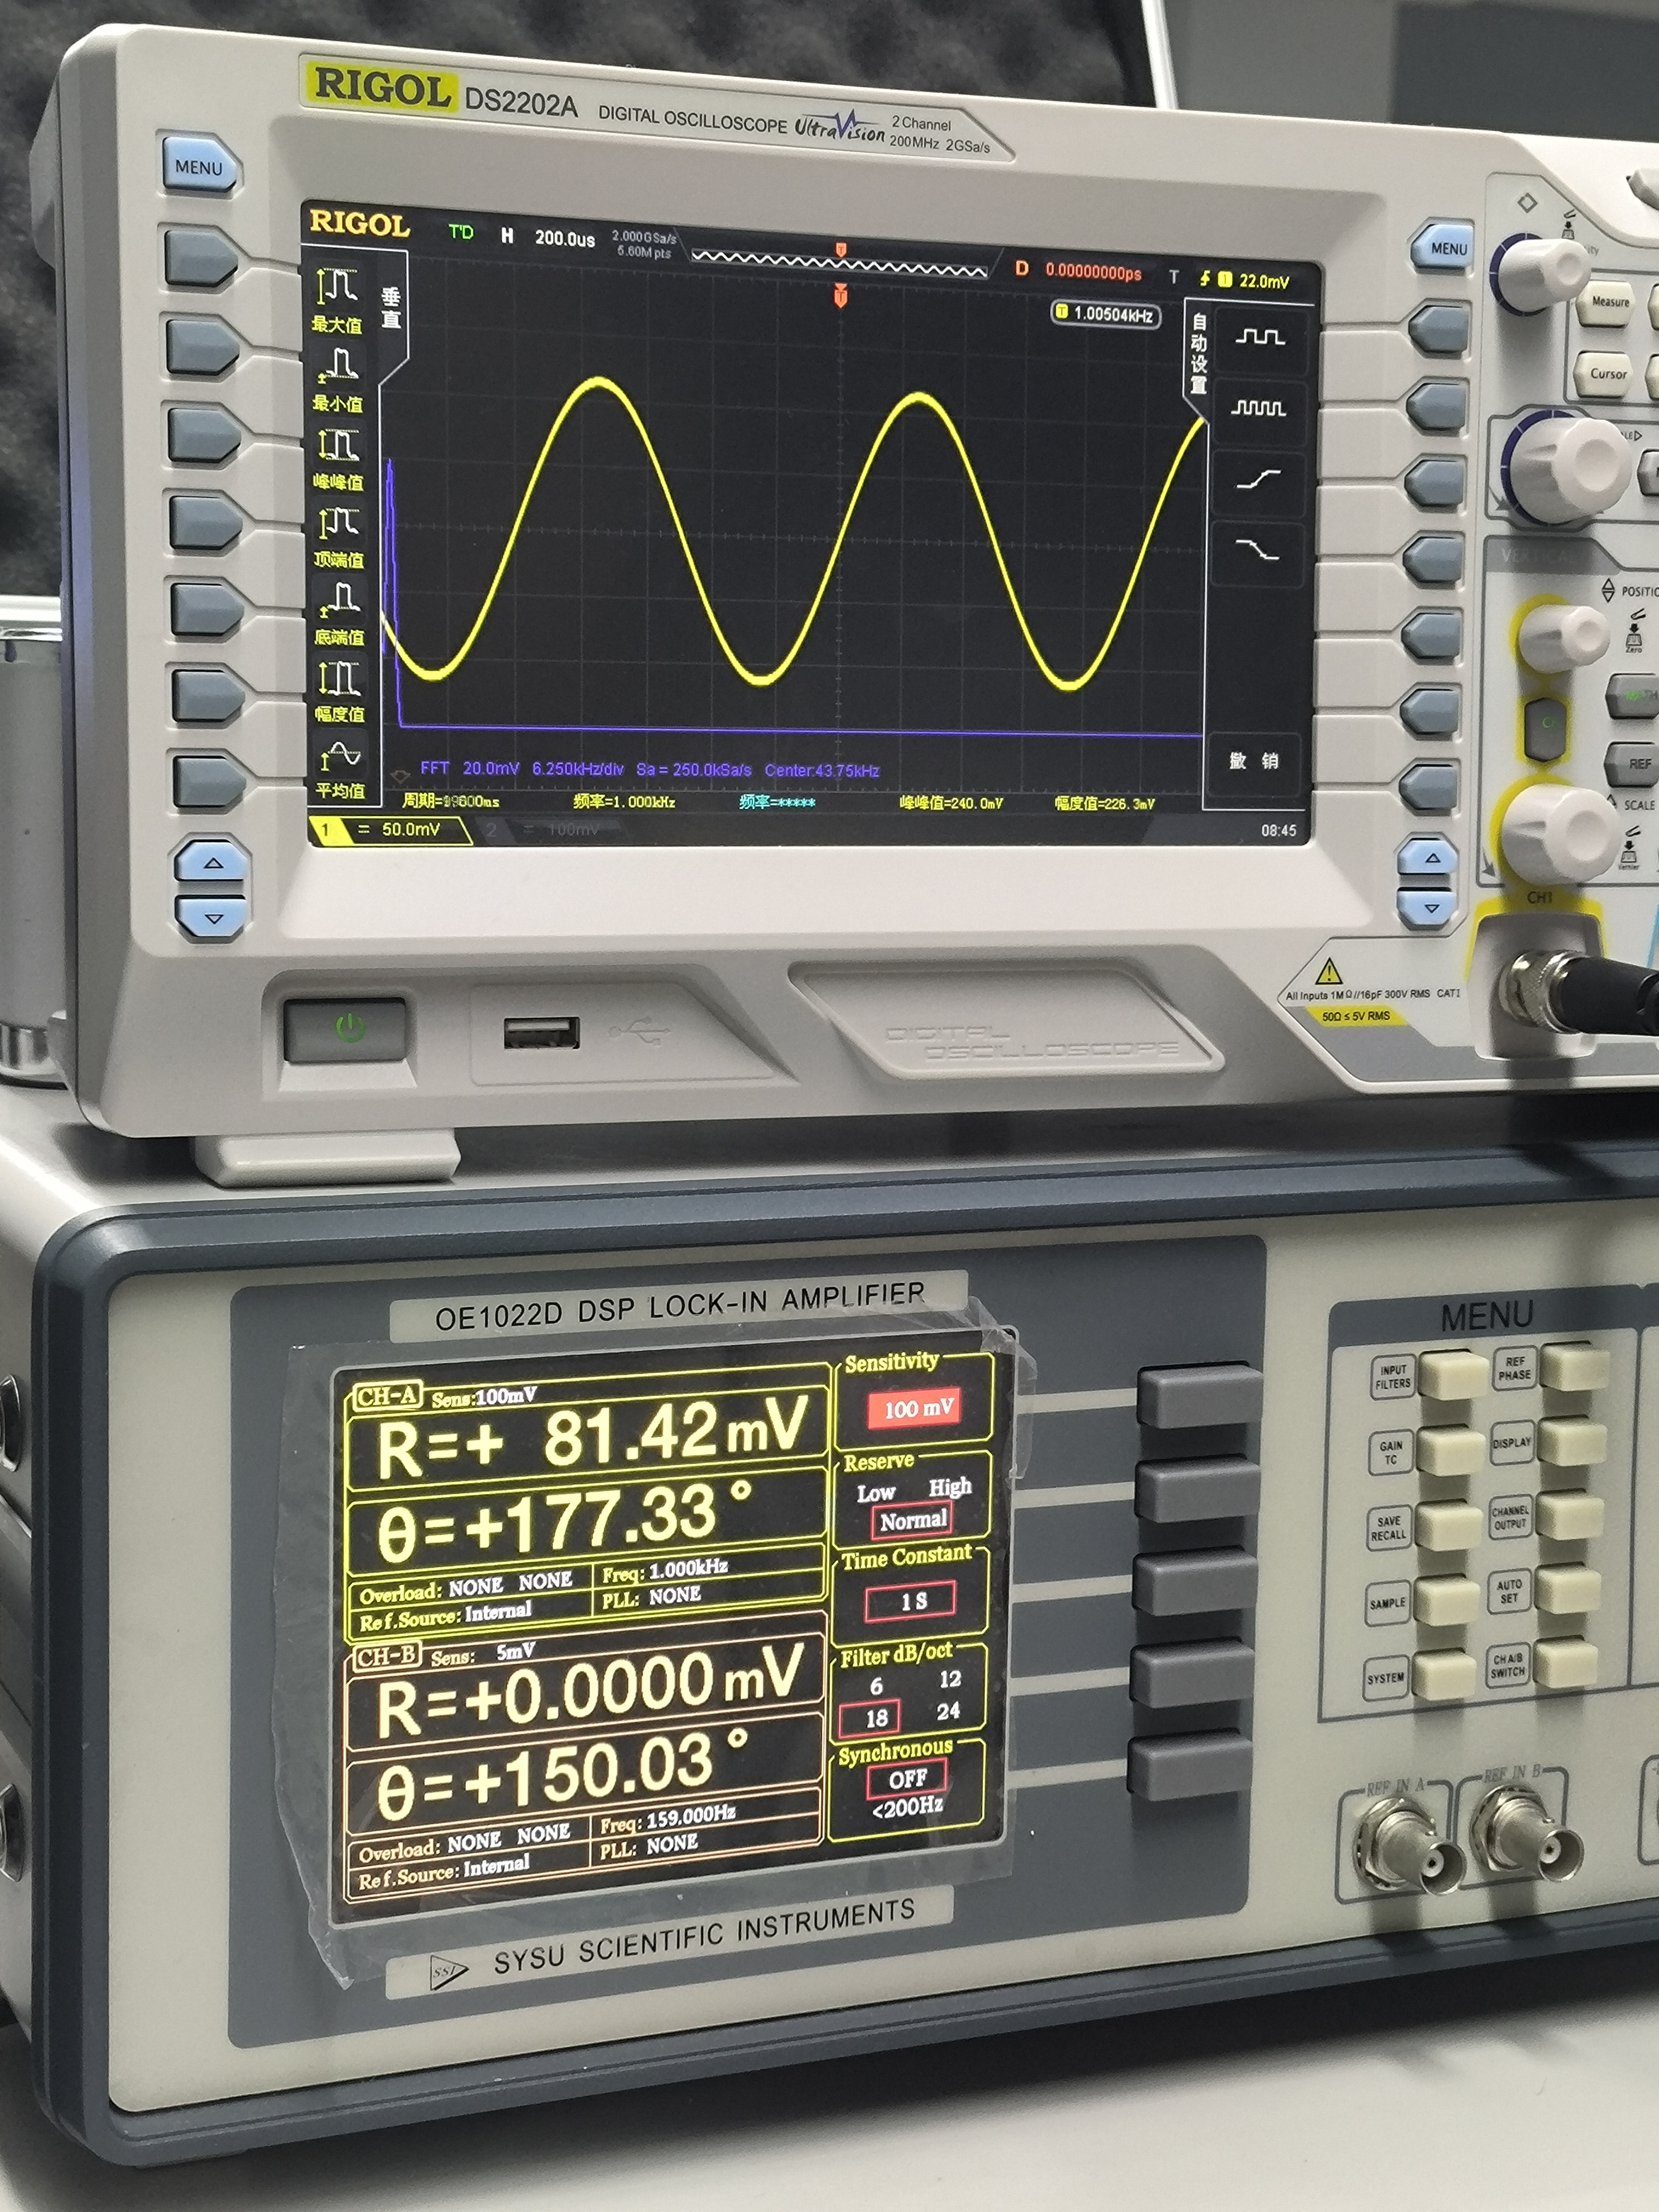
\includegraphics[width=0.5\textwidth]{D1-1-1.jpg}
		\caption{用示波器观察内部信号输出}
		\label{fig:D1-1-1}
	\end{wrapfigure}

	在锁相放大器的“SineOutput”中设置“Voltage = 80mVrms”,频率设置为1kHz,即可产生一个正弦波,图像如\cref{fig:D1-1-1}。

	通过示波器测量到的信号确实为正弦波,测量的峰峰值$V_{pp} = 240.0 \text{mV}$,频率$f = 1.000 \text{kHz}$。

	% 即测量的有效值为$$V_{rms} = \frac{V_{pp}}{2\sqrt{2}} = 84.85 \text{mV}$$ 与设定值$80 \text{mV}$之间有一定误差;



	\clearpage
	\subsubsection{测量信号 $R$、$\theta$、$X$以及$Y$值,并验证它们之间的关系}


	\begin{table}[htbp]
		\centering
		\begin{tabular}{|llll|} 
		\hline
		$R/\text{mV}$  & $X/\text{mV}$   & $Y/\text{mV}$ & $\theta/°$  \\ 
		\hline
		81.43 & -81.34 & 3.79 & 177.33   \\
		\hline
		\end{tabular}
		\caption{测量信号的 $R$、$\theta$、$X$、$Y$值}
		\label{tbl:D1-2-1}
	\end{table}

	通过前面板DISPLAY按键,测量实时显示的$R$、$\theta$、$X$、$Y$值,结果如\cref{tbl:D1-2-1}







	\subsubsection{相敏检波器工作原理——乘法器}

	将锁相放大器设置为内部参考信号,耦合方式设置为DC,将滤波器带宽调至最大(即$TC = 10 \mu\text{s}, \text{Slope} = 6 \text{dB/cot}$),观察锁相放大器的模拟输出的$R$信号的波形,如\cref{fig:D1-3-1}所示;同时观察$X$,$Y$信号的波形,如\cref{fig:D1-3-2}所示。

	\begin{figure}[htbp]
		\centering
		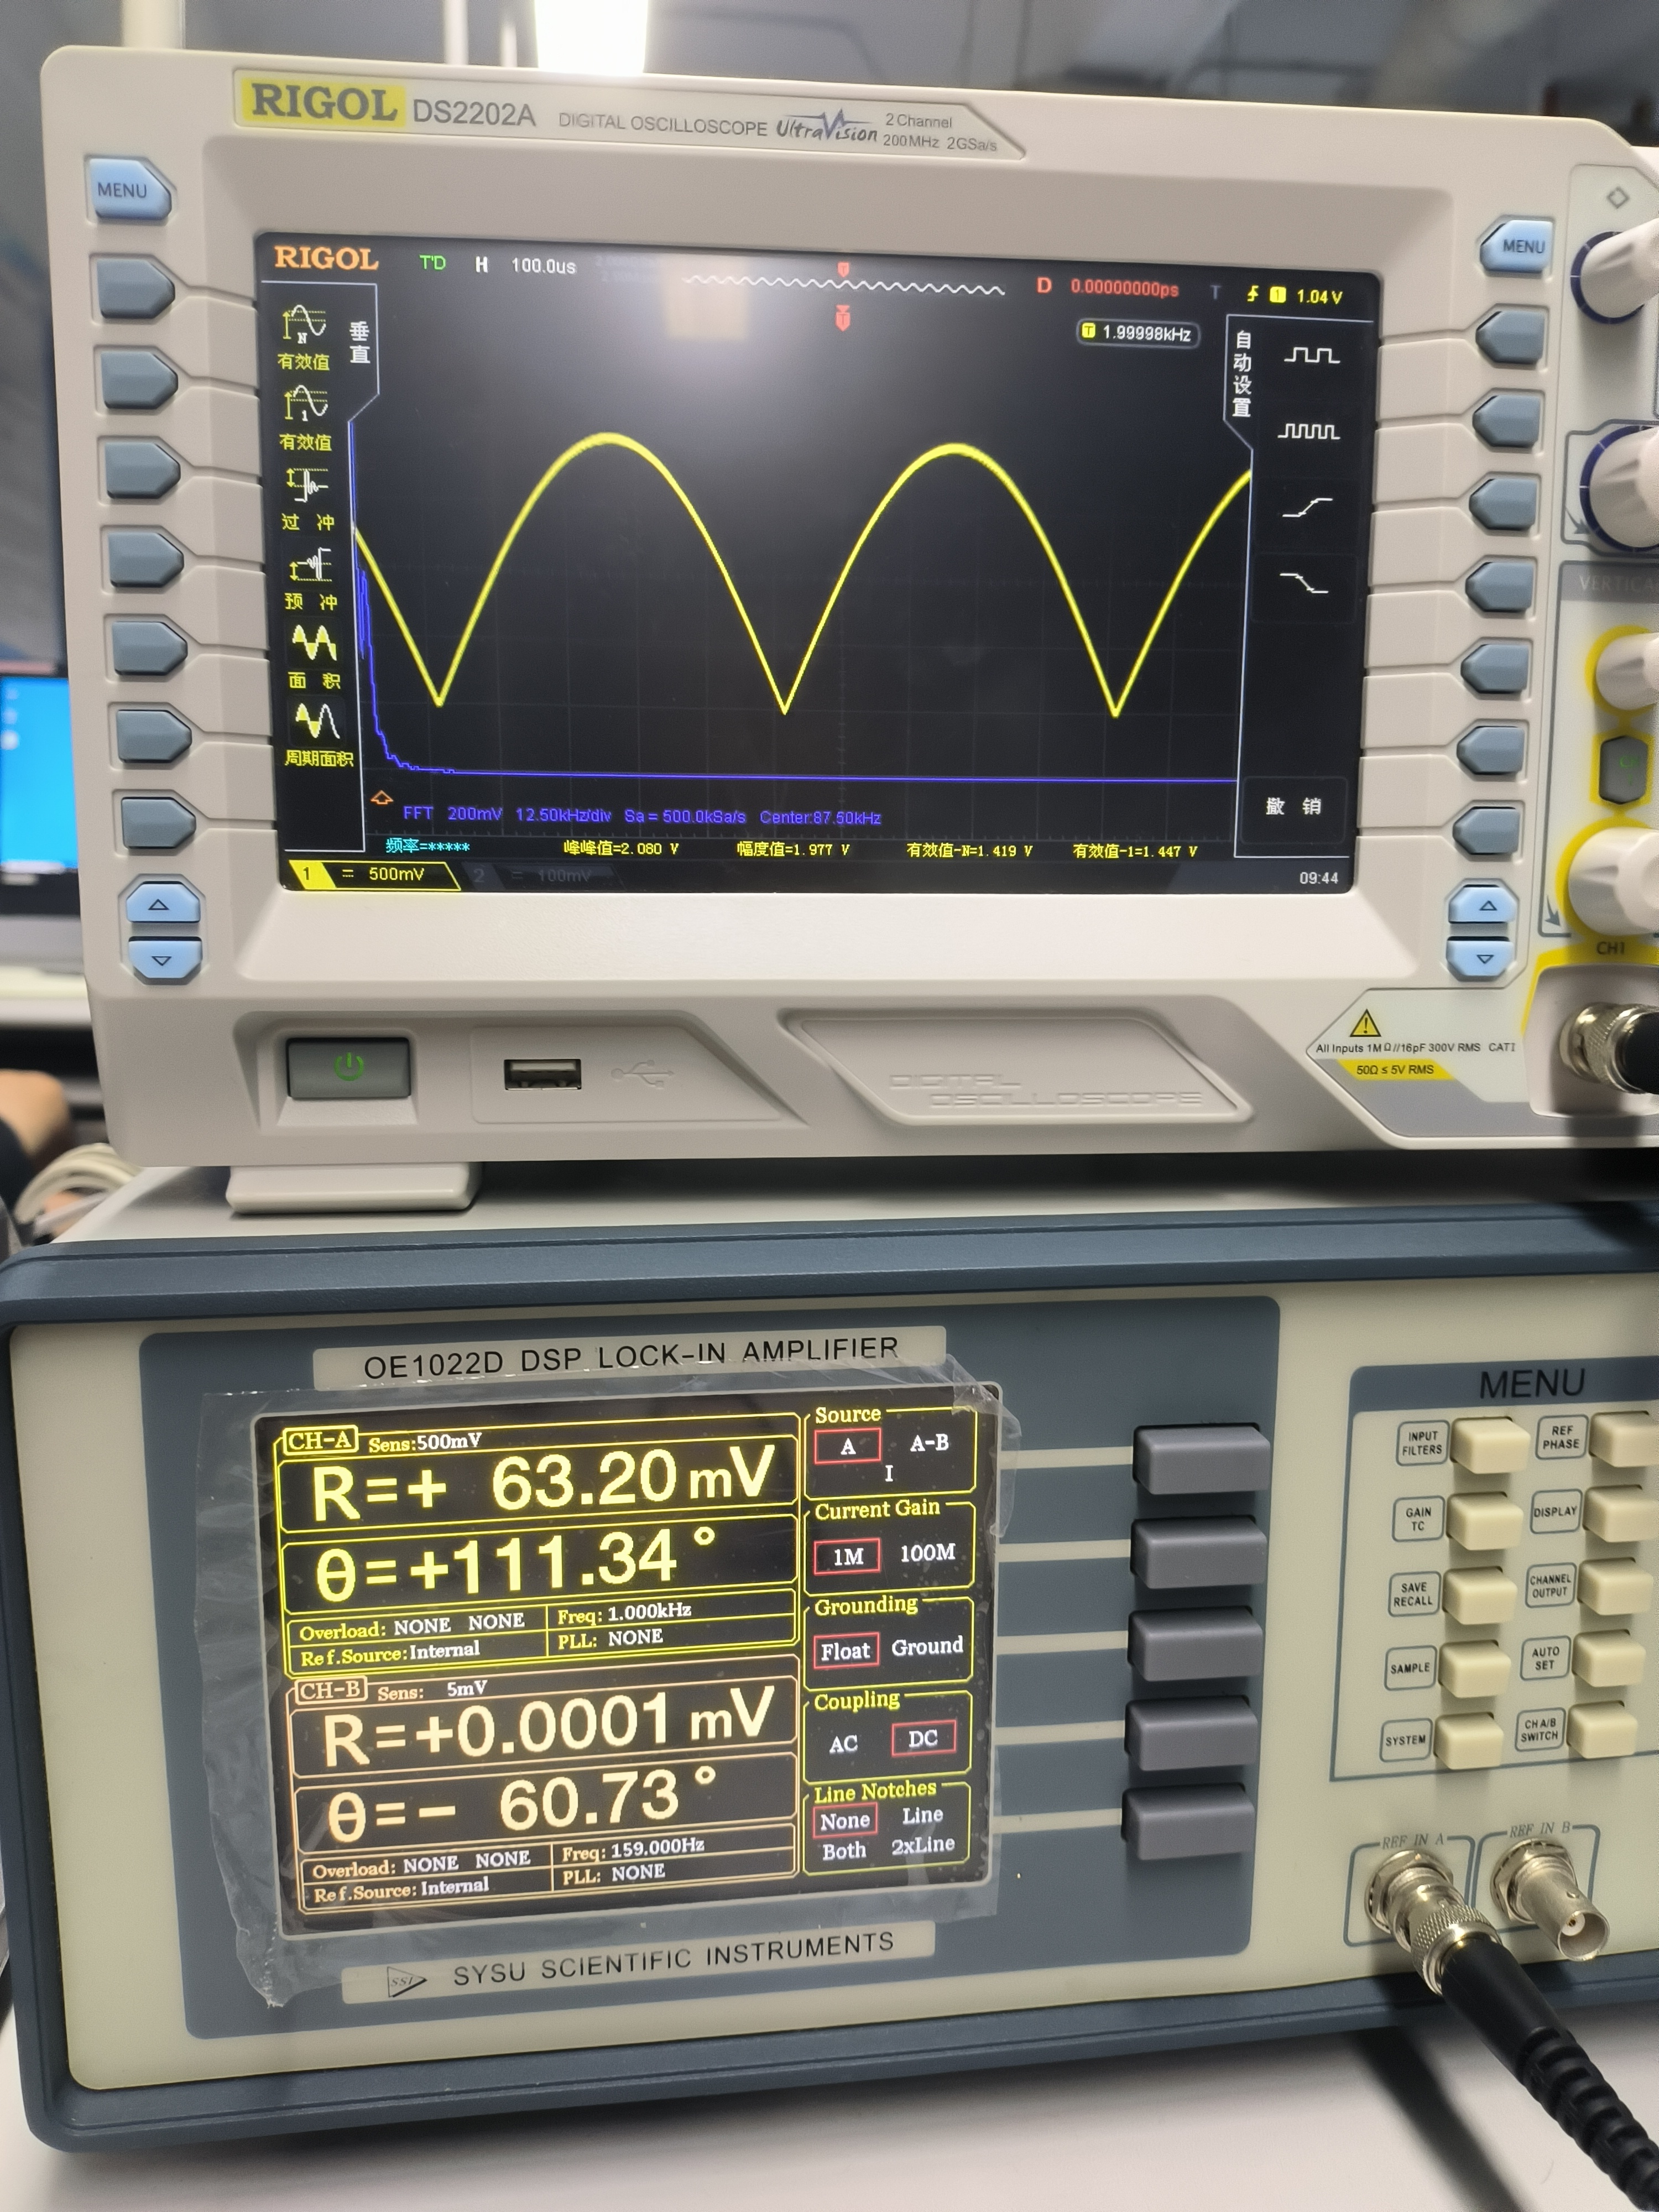
\includegraphics[width=0.6\textwidth]{D1-3-1.jpg}
		\caption{乘法器输出的$R$的图像}
		\label{fig:D1-3-1}
	\end{figure}


	\begin{figure}[htbp]
		\centering
		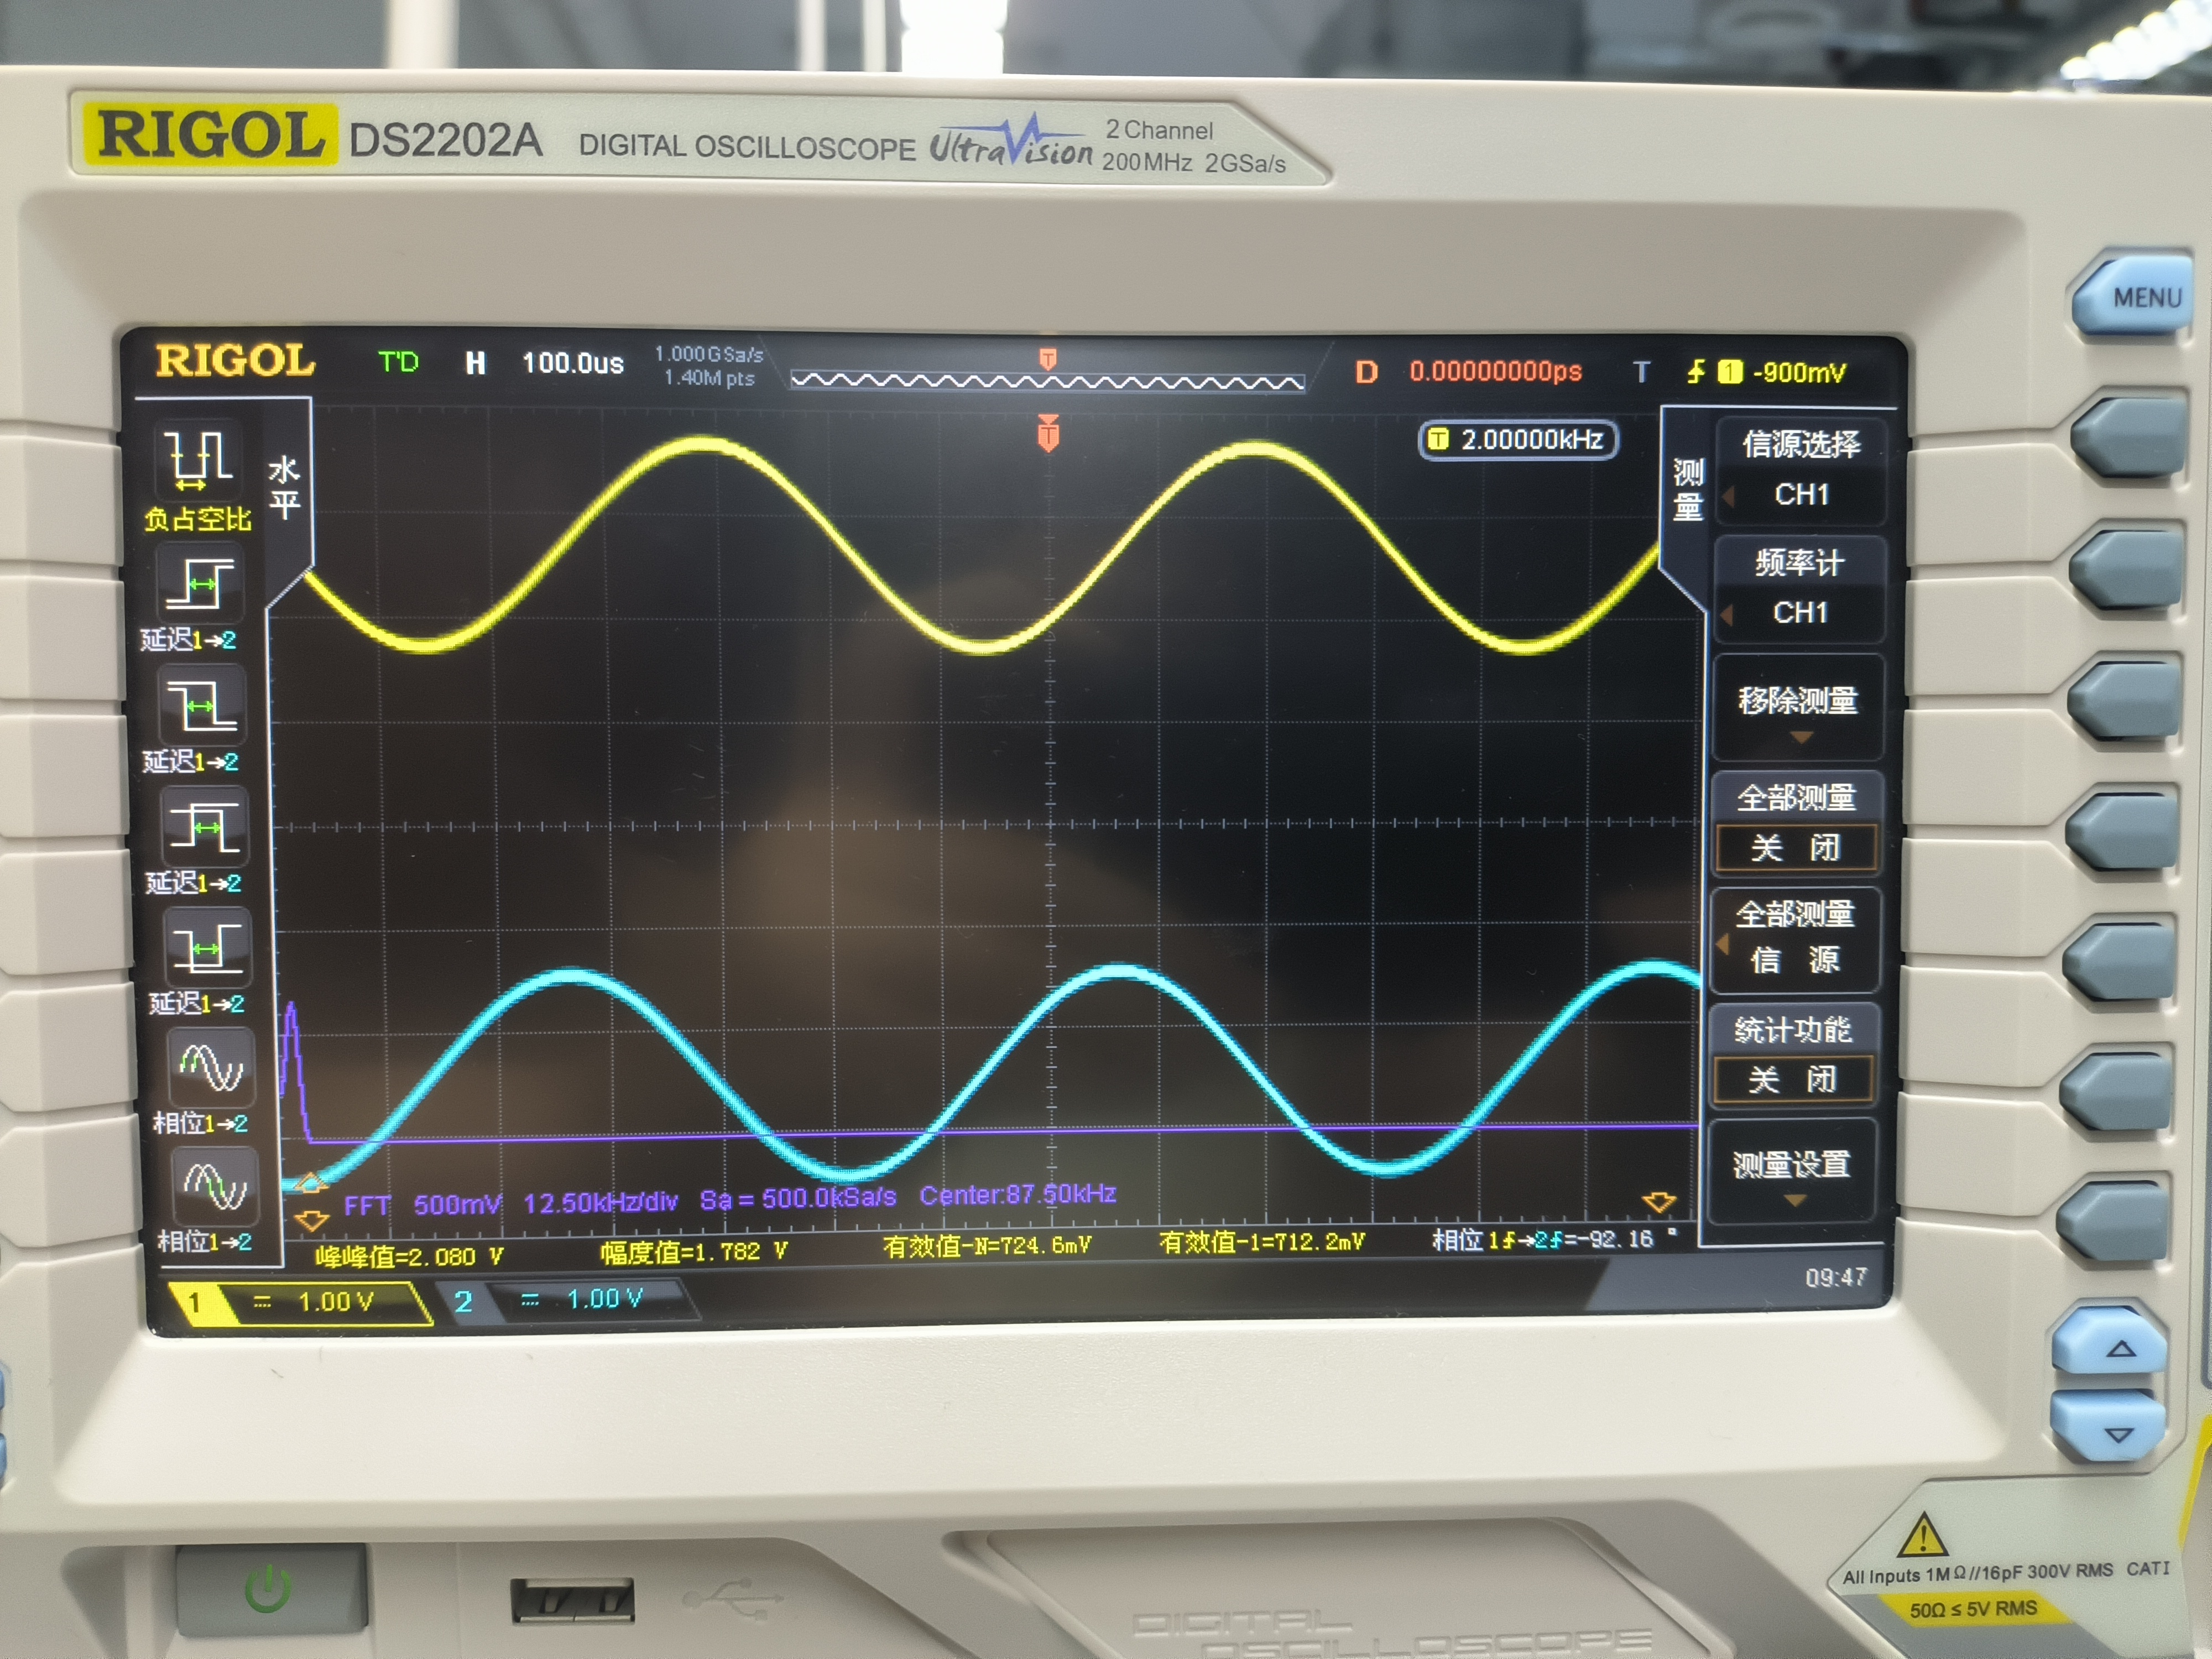
\includegraphics[width=0.6\textwidth]{D1-3-2.jpg}
		\caption{乘法器输出的$X$,$Y$的图像}
		\label{fig:D1-3-2}
	\end{figure}







	\subsubsection{相敏检波器工作原理——乘法器+低通滤波器}

	对锁相放大器的滤波器设置不同的时间常数和陡降,通过示波器观察锁相放大器的输入信号波形、乘法器输出的$R$,$X$,$Y$波形,同时记录锁相放大器的$R$,$X$,$Y$读数。













	\subsubsection{强噪声背景下的弱信号检测}

	实验过程中,首先测量噪声发生器的噪声信号有效值约为120.1mV,如\cref{fig:D1-8-1}所示。通过该值

	\begin{figure}[htbp]
		\centering
		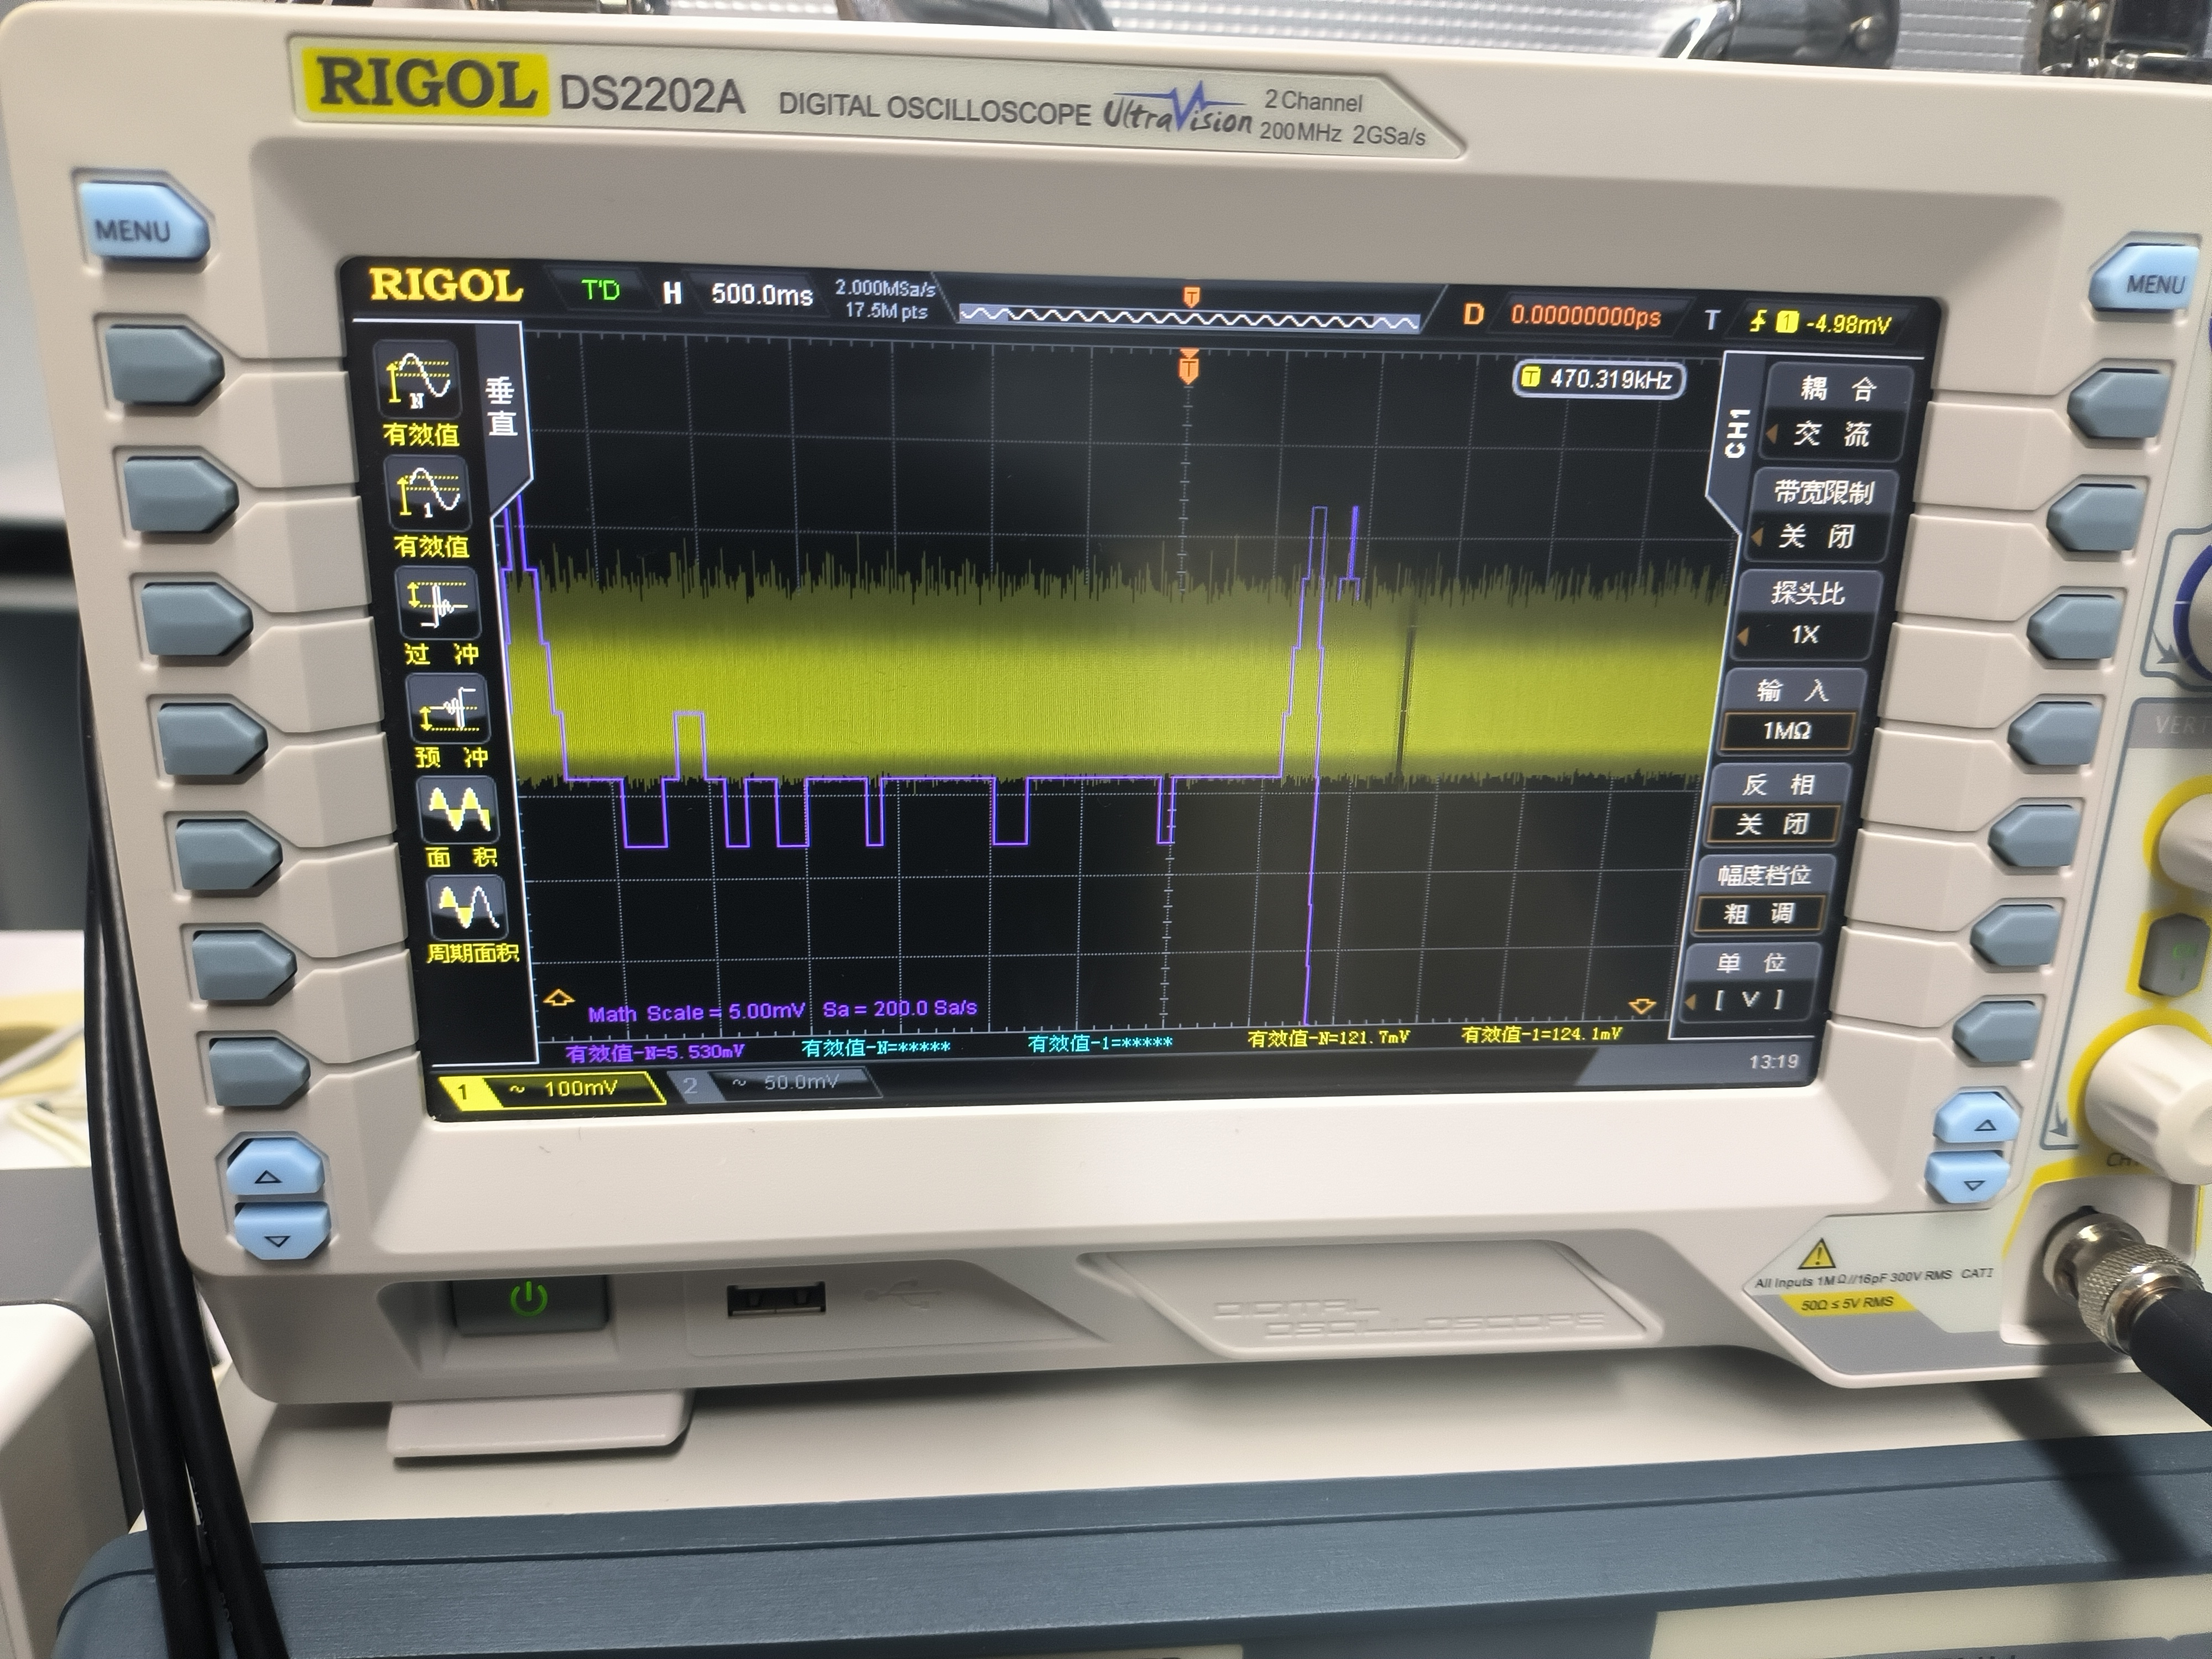
\includegraphics[width=0.6\textwidth]{D1-8-1.jpg}
		\caption{噪声发生器的噪声信号测量}
		\label{fig:D1-8-1}
	\end{figure}

	\begin{table}[htbp]
		\centering
		\begin{tblr}{
		  cells = {c},
		  cell{2}{1} = {r=6}{},
		  cell{8}{1} = {r=7}{},
		  vline{1-2,4,7} = {-}{},
		  vline{4,7} = {3-7,9-14}{},
		  hline{1-2,8,15} = {-}{},
		}
		仪器    & 输入信号信噪比    & dB     & 0            & -30          & -80      \\
		示波器   & 正弦波$V_{in}$幅值 & mVrms  & 119.2        & 3.8          & -        \\
			  & 噪声信号大小     & mVrms  & 120.7        & 120.7        & 120.7    \\
			  & SNRi       & dB     & -0.11 & -30.04 & -80 \\
			  & 滤波器带宽      & Hz     & 1000         & 1000         & 1000     \\
			  & 滤波后信号有效值   & mVrms  & 135          & 4.8          & -        \\
			  & SNRo,os   & dB     & 0.97  & -28.01 & - \\
		锁相放大器 & 量程灵敏度      & mV     & 200          & 20           & 20       \\
			  & 时间常数       & ms     & 10           & 300          & 300      \\
			  & 陡降         & dB/oct & 24           & 24           & 24       \\
			  & LPF带宽      & Hz     &              &              &          \\
			  & 信号有效值R     & mVrms  & 120.1        & 3.77         & 12.1     \\
			  & 噪声有效值N     & mVrms  & 0.02         & 0.028        & 0.106    \\
			  & SNRo,lo    & dB     & 75.57  & 42.58  & 41.15  
		\end{tblr}
		\caption{强噪声背景下的弱信号检测数据}
		\label{tbl:D1-8-1}
	\end{table}



\subsection{实验数据记录}

	% 见\cref{fig:data}

	% \begin{figure}[htbp]
	% 	\centering
	% 	\subfloat[原始数据1]
	% 	{\includegraphics[width=0.35\textwidth]{OriginalData1.jpg}\label{fig:data1}}
	% 	\quad
	% 	\subfloat[原始数据2]
	% 	{\includegraphics[width=0.35\textwidth]{OriginalData2.jpg}\label{fig:data2}}
	% 	\quad


	% 	\caption{原始数据}
	% 	\label{fig:data}
	% \end{figure}



%\subsection{原始数据记录}



\subsection{实验过程中遇到的问题记录}

\begin{enumerate}
	\item 
	
\end{enumerate}
	

\clearpage
\begin{table}
	\renewcommand\arraystretch{1.7}
	\begin{tabularx}{\textwidth}{|X|X|X|X|}
	\hline
	专业:& 物理学 &年级:& 2022级\\
	\hline
	姓名: & 戴鹏辉 & 学号:& 22344016\\
	\hline
    日期:& 2024/5/12 & 评分: &\\
	\hline
	\end{tabularx}
\end{table}

\section{D1 \quad 锁相放大器与弱信号测量 \quad\heiti 分析与讨论}

\subsection{实验数据分析}


	\subsubsection{实验一 \quad 选择合适电流量程,设置氩管工作电压}
		
		





\end{document}
